\chapter{実装}\label{cha:Implementation}

本章では、本研究で試作したモータ特性表自動生成ツールの実装について説明する。

% \section{特性表生成機能}\label{tokuseihyou_seisei}

% モータ特性表自動生成ツールの処理の流れを図\ref{fig:syori}に示す。\\

% \begin{figure}[t]
% 	\centering
% 	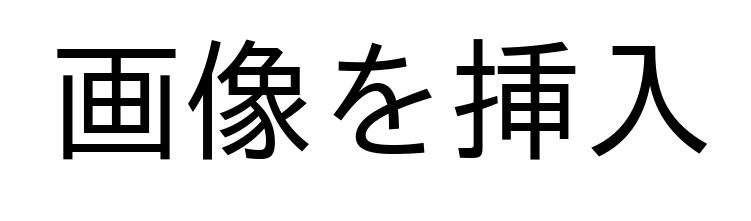
\includegraphics[width=16.5cm,height=10cm]{./Image/sample.png}
% 	\caption{モータ特性表自動生成ツールの処理の流れ}
% 	\label{fig:syori}
%   \end{figure}

特性表生成機能の処理の流れを以下に示す。
\begin{enumerate}
    \item OpenModelicaから出力されたcsvファイルを読み込む
    \item 特性表の各要素を算出するために必要なデータを、csvファイルから取得する
    \item 特性表の各要素を算出する
    \item 特性表を生成する
\end{enumerate}

以下、各処理について具体的に説明する。

\section{csvファイルの読み込み}\label{csvfairu}
Pythonで実装するため、Pythonの標準ライブラリのcsvモジュールをインポートし、
csvファイルを読み込む。

\section{特性表の各要素を算出するために必要なデータを取得}\label{syutoku_data}
\ref{csvfairu}節で読み込んだcsvファイルから、以下のデータを取得する。

\begin{itemize}
    \item 時間
    \item 電流
    \item 電圧
    \item トルク
    \item 角速度
\end{itemize}

図\ref{fig:simyu_csv}に示したように、OpenModelicaから出力されたcsvファイルの1行目には、
各部品の変数名が記載されている。これを利用して、次の処理で必要なデータを取得する。

\begin{enumerate}
    \item 
\end{enumerate}
取得したいデータを持つ変数名を探し、その変数名がある場所の添字を取得する。
各データごとに用意した配列に、同じ添字の位置にある値を繰り返し処理で格納する方法でそれぞれの値を取得する。

\section{特性表の各要素を算出}\label{keisan}
\ref{syutoku_data}節で取得したデータを用いて、\ref{kenkyu_mokuteki}節で挙げた各要素の値を求める。

\subsection{電圧}\label{sub:keisan_dennatu}
% シミュレーション時に印加した値を取る。

\subsection{始動電流}\label{sub:keisan_sidouden}
% 始動電流とは、モータの起動時に流れる大きな電流のことである。
% モータが起動した後はモータ自体が発電機にもなり、逆起電力を発生するため、モータ・コイル部分にかかる電圧が下がり、電流値も下がる。
% したがって、電流値の配列の中で一番大きい値を始動電流とする。

% https://www.tsugawa.co.jp/glossary/ 

\subsection{停動トルク}\label{sub:keisan_teidoutoruku}
% 停動トルクとは、モータが出しうる最大トルクで、このトルク以上の負荷がかかれば、モータは停止する値となる。
% したがって、トルク値の配列の中で一番大きい値を停動トルクとする。

% https://www.orientalmotor.co.jp/tech/glossary/ta11/

\subsection{最大効率}\label{sub:keisan_saidaikouritu}
% 効率は以下の式で算出することができる。

% \[
%     \mbox{効率} = \frac{\mbox{出力}}{\mbox{入力}}  * 100 
% \]
% \[
%     \mbox{出力} = \mbox{角速度} * \mbox{トルク} 
% \]
% \[  
%     \mbox{入力} = \mbox{電圧} * \mbox{電力} 
% \]

% 各配列を上記の式に当てはめ、繰り返し処理で効率値の配列を作成する。
% 最大効率は効率値の配列の中で一番大きい値とする。

% https://www.jp-igarashi.com/product/product_motors/curve.html

\subsection{定格トルク}\label{sub:keisan_teikakutoruku}
% 最大効率時のトルクを定格トルクという。
% したがって、トルク値の配列の中で、最大効率のある効率値の配列の添字と同じ位置にある値が定格トルクとなる。


% http://www.sagamimicro.co.jp/product/aboutusage.html

\subsection{定格回転数}\label{sub:keisan_teikakukaiten}
% 最大効率時の回転数を定格回転数という。
% 回転数は以下の式で算出できる。

% \[
%     \mbox{回転数} = \frac{30 * \mbox{角速度}}{\pi}   
% \]

% したがって、一度繰り返し処理で角速度を回転数に変換し、回転数値の配列の中で、最大効率のある効率値の配列の添字と同じ
% 位置にある値が定格回転数となる。

% https://mathwords.net/kaitensu

\subsection{定格電流}\label{sub:keisan_teikakuden}
% 定格電流とは、モータに定格トルクがかかっているときの電流値である。
% したがって、電流値の配列の中で、定格トルクのあるトルク値の配列の添字と同じ位置にある値が定格電流となる。

% http://fa-faq.mitsubishielectric.co.jp/faq/show/18504?category_id=1937&site_domain=default

\subsection{定格出力}\label{sub:keisan_teikakusyutu}
% 定格出力とは、定格動作点における出力の値である。
% 定格出力は以下の式で算出できる。

% \[
%     \mbox{定格出力} = \mbox{定格回転数} * \mbox{定格トルク} *  \frac{2\pi}{60}
% \]
% \ref{sub:keisan_teikakukaiten}章で求めた定格回転数と\ref{sub:keisan_teidoutoruku}章で求めた定格トルクを
% http://www.nidec-servo.com/jp/digital/pdf/A_technique.pdf

\section{特性表を生成}\label{seisei_hyou}
\ref{keisan}章で求めた各値と、\ref{kenkyu_mokuteki}章で挙げた各要素を、電圧から順に","で区切りつつ
特性表生成配列に格納する。そして特性表生成配列を用いてcsvファイルを作成する。

